%%%%%%%%%%%%%%%%%%%%%%%%%%%%%%%%%%%%%%%%%%%%%%%%%%%%%%%%%%%%%%%%%%%%
% Introduction
%%%%%%%%%%%%%%%%%%%%%%%%%%%%%%%%%%%%%%%%%%%%%%%%%%%%%%%%%%%%%%%%%%%%
\onehalfspacing
\chapter{Introduction}
\label{Introduction}
Trello is a webservice by the New York City based web corporation Fog Creek Software\footnote{Official Fog Creek Software website: \url{http://www.fogcreek.com}}\index{Fog Creek Software}. It is a collaboration tool to manage projects and was launched in 2011\footnote{The original launch post in the Trello blog: \url{http://blog.trello.com/launch/}}. 

\begin{figure}[htb]
\centering
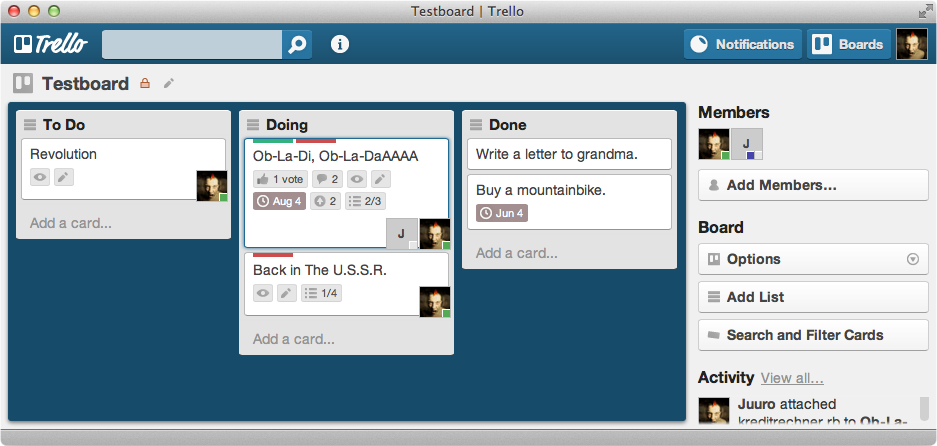
\includegraphics[width=\textwidth]{figures/trello}
\caption{A Trello board.}
\label{fig:trello}
\end{figure}

The sevice focuses on the concept of so called \emph{boards} containing several configurable lists. Figure \ref{fig:trello} shows a board with the three standard lists \emph{To Do}, \emph{Doing}, and \emph{Done}. In these lists, the user can create to-do items called \emph{cards} containing additional data. Each card has a title and an optional description, some assigned members, a due date, some labels, votes, checklists, comments, and attachments. The creator of the board is the owner and can add other Trello users to his boards and cards. This way, everone who's working on a project can see what is going on at the moment. Users who are assigned to a board can even create new to-do items by themselves. If it should be the case that somebody works at more than one company with many projects each, there is the concept of \emph{organizations} to ensure clear separation.

It is possible to manage complete projects within Trello, but sometimes the information in Trello should be displayed in a different manner. For example if there are due dates managed by Trello. It would be useful to display them in the calendar application the user uses otherwise. Trello can't provide information to other applications or web services itself. To work with data outside of Trello, there is a API to access all kinds of data in Trello. This thesis represents the Trello API in Ruby, and extends it with useful methods to allow developers a convenient possibility to access Trello.

The thesis is organised as follows: The basics are discussed in Chapter \ref{Principles}. This mainly includes a description of the collaboration tool Trello, a brief introduction to the Ruby programming language and the explanation of the used formats and procedures. Chapter \ref{apiwrapper} deals with the development of an API wrapper in Ruby for the Trello API. Here, the most important methods are described in detail. In the \hyperref[applications]{applications section} the API wrapper is used to link Trello to other services and to extract application-specific data from Trello respectively add new information to Trello. A discussion and a brief outlook on further possible applications of the API wrappers in Chapters \ref{Conclusion} and \ref{Outlook} conclude this thesis.